\documentclass[tikz,border=10pt]{standalone}
\usetikzlibrary{positioning}
\usepackage{tkz-graph}
\usepackage{rotating}
\usetikzlibrary{arrows}
\usetikzlibrary{arrows.meta}

\begin{document}

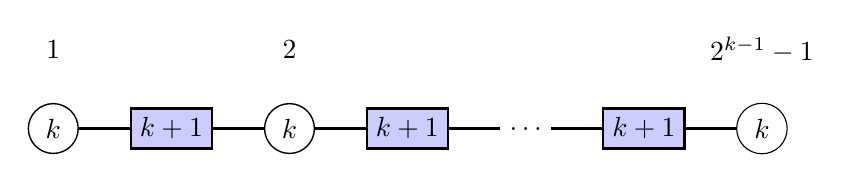
\begin{tikzpicture}
\SetGraphUnit{3}
\tikzset{LabelStyle/.style= {draw, fill = blue!20}}
\Vertex[L=$k$]{A}
\EA[L=$k$](A){B}
\tikzset{VertexStyle/.style = {draw=none,fill=none, text = black}}
\EA[L=$\ldots$](B){C}
\tikzset{VertexStyle/.style = {shape=circle, text = black, draw}}
\EA[L=$k$](C){D}
\Edge[label=$k+1$](A)(B)
\Edge[label=$k+1$](B)(C)
\Edge[label=$k+1$](C)(D)
\draw node [above of=A] {$1$};
\draw node [above of=B] {$2$};
\draw node [above of=D] {$2^{k-1}-1$};
\end{tikzpicture}

\end{document}